% !TEX root=../main.tex

\section{Attention and Anticipation}\label{sec:anticipation}

The attention and anticipation algorithm~\cite{Carlone2017} selects a subset $\mathsf{S}$ of the features $\mathsf{F}$ detected in the current frame to pass to the VIO back end.
The subset of features should have at most $\kappa$ features that are the most useful for reducing uncertainty in vision-based state estimation.
This feature selection problem can be stated as
\begin{equation}\label{eqn:sensor-selection-problem}
\max_{\mathsf{S}\subset\mathsf{F}} \quad f(\mathsf{S}) \qquad \text{subject to}\quad |\mathsf{S}|\le\kappa.
\end{equation}
The solution of this problem relies on the selection of a metric $f$ that maps subsets of features to their usefulness.

Although sensor selection problems have been shown to be NP-hard because of the introduction of binary selection variables, recent results have leveraged submodular cost functions to allow greedy algorithms to find efficiently solutions to Problem~\eqref{eqn:sensor-selection-problem} with guarantees on suboptimality~\cite{Shamaiah2010}.
\pcl{define what a submodular set function is.}
The goal then is to identify a performance metric that exhibits submodularity and captures the accuracy of VIO.

Following~\cite{Carlone2017}, we use the logdet metric to measure the volume of the estimation uncertainty ellipsoid up to scaling.
Let $k+1$ be the time at which we have obtained a new feature set to choose from.
Then $\x_k$ is the optimized pose of the previous camera frame, which is the latest pose estimate from the fixed-lag smoother of the pose-graph optimization back end (see Figure~\ref{fig:meas_timeline}).
Let $\xhatkkH\triangleq\begin{bmatrix}\x_k&\xhat_{k+1}&\cdots&\xhat_{k+H}\end{bmatrix}$ denote the stacked state vector over a horizon $H$, where $\xhat_{k+1:k+H}$ are predicted future states yet to be optimized over.
Moreover, let $\PkkH$ be the covariance of the estimation error corresponding to $\xhatkkH$ and its inverse is called the information matrix, denoted $\OmegakkH\triangleq\PkkH^{-1}$.
With these definitions, the logdet metric is written
\begin{align}
\fdet(\mathsf{S}) &= \logdet(\OmegakkH(\mathsf{S}))\\
&= \logdet\left(\OmegabarkkH + \sum_{l\in\mathsf{S}}p_l\Delta_l\right),
\end{align}
where $\OmegabarkkH$ is the information matrix corresponding to the predicted robot motion over the horizon and $\Delta_l$ is the information matrix of the $l$-th feature.
The remainder of this section discusses the computation of $\OmegabarkkH$ and $\Delta_l$, and the implementation of the greedy selection algorithm.

\begin{figure}
\centering
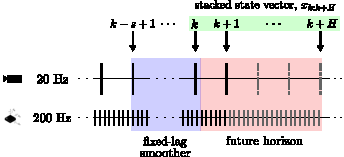
\includegraphics[width=\columnwidth]{meas_timeline.pdf} 
\caption{Timing diagram.}
\label{fig:meas_timeline} 
\end{figure}


% =============================================================================
\subsection{Attention Allocation Algorithm for Feature Selection}\label{sub:attn_algo}

The following greedy algorithm is used to approximately solve Problem~\eqref{eqn:sensor-selection-problem} by selecting $\kappa$ features that (approximately) maximize the logdet metric.
As input, it takes the number of features to select ($\kappa$), the anticipated information from future robot motion ($\OmegabarkkH$), the anticipated information from each new landmark ($\{\Delta_l\}_{l\in\mathsf{F}}$), and the current information of existing landmarks ($\{\Delta_l'\}_{l\in\mathsf{F}'}$).
The following subsections will discuss how to obtain these information matrices.

The greedy algorithm with lazy evaluation involves the following steps. 
\begin{enumerate}
    \item The algorithm takes in $\bar{\Omega}_{k:k+H}$ (the $9(H+1)$ x $9(H+1)$ information matrix of the future states based solely on IMU and features already seen rather than new features) and $\Delta_l$ (the $9(H+1)$ x $9(H+1)$ x (num of features) information matrix of the future states associated with the l'th feature).
    \item For each iteration over the number of features desired in the subset, upper bounds are computed that bounds the information gained by adding each feature to the current subset.
    \item After initializing the variables $f_{max}$ and $l_{max}$, we check if the upper bound is less than the current $f_{max}$ for each landmark in the sorted upper bound list; if so, we break on the for loop and and select the currently best feature (lazy evaluation). If the upper bound is greater than the current $f_{max}$, we calculate the objective function of the new proposed subset by adding that particular feature to the current subset; if it is greater than the current $f_{max}$, we keep track of this value for the next iteration, ultimately keeping track of the maximum $f_{max}$ for the feature that adds the most information to the current subset.
    \item This feature is added to the subset, and the iteration continues until $\kappa$ features are added to the subset.
\end{enumerate}
Now we will look into how to calculate the information matrices.


% =============================================================================
\subsection{Anticipated Information from Robot Motion}\label{sub:info_motion}

$\bar{\Omega}_{k:k+H}$ is given by the following equation.
\begin{equation}
    \bar{\Omega}_{k:k+H} = \bar{\Omega}_{k:k+H}^{IMU} + \bar{\Omega}_{k:k+H}^{PRIOR}
    \label{eq:omega_IMU}
\end{equation}
Thus, we need to find $\bar{\Omega}_{k:k+H}^{IMU}$ and $\bar{\Omega}_{k:k+H}^{PRIOR}$. To find $\bar{\Omega}_{k:k+H}^{PRIOR}$, we know it is a $9(H+1)$ x $9(H+1)$ matrix that is 0 everywhere except for the top left block which is the prior on state k, $\bar{\Omega}_{k}^{PRIOR}$. This is found by retrieving the covariance of the state estimate at time k from the pose graph and inverting it to give the information matrix at time k. ($\bar{\Omega}_{k:k+H}^{PRIOR}$). \\ \\
Next to find $\bar{\Omega}_{k:k+H}^{IMU}$, we use the following equation, which comes from the future IMU preintegration that is used to sum up IMU information from consecutive frames. 
\begin{equation}
    \bar{\Omega}_{k:k+H}^{IMU} = \sum_{kj \in H} (A^T_{kj}\bar{\Omega}_{kj}^{IMU}A_{kj})
\end{equation}
We assemble $A_{kj}$ as follows from the linearized dynamic model, where the position of $I_9$ is always the next consecutive frame from $k$ such that it is on the $(k+1)$th block.
\[
\begin{bmatrix}
    0_{9x9} ... & A_{k} & I_9 & 0_{9x9} ... \\
\end{bmatrix}\]

where $A_{k}$ is given below.
\[A_{k} = 
\begin{bmatrix}
-I_3 & -I_3\delta_{kj} & N_{kj} \\
0 & -I_3 & M_{kj} \\
0 & 0 & -I_3 \
\end{bmatrix}\]
To find $N_kj$ and $M_kj$ in $A_{block}$, we use the following equations. 
\begin{equation}
    N_{kj} = \sum_{i=k}^{j-1}(j-i-\frac{1}{2})R_i\delta**2
\end{equation}
\begin{equation}
    M_{kj} = \sum_{i=k}^{j-1}R_i\delta
\end{equation}
Next, to find $\Omega_{kj}^{IMU}$, we see that this is the information matrix associated with the noise $\eta_{kj}^{IMU}$. The equation for this is given below. 
\[\Omega_{kj}^{IMU} = (cov(\eta_{kj}^{IMU}))^{-1} =
\begin{bmatrix}
\sigma_{IMU}^2CC^T & 0_{6x3} \\
0_{3x6} & cov(\eta_{kj}^b) \\
\end{bmatrix}
\]

Instead of calculating $CC^T$ through matrix multiplication, we can directly calculate each block entry as per the equation below.
\[CC^T =
\begin{bmatrix}
(\sum_{i=k}^{j-1}(j-i-\frac{1}{2})^2)\delta^4 I_3 & (\sum_{i=k}^{j-1}(j-i-\frac{1}{2}))\delta^3 \\
(\sum_{i=k}^{j-1}(j-i-\frac{1}{2}))\delta^3  &
(j-k-1)\delta^2I_3 \\
\end{bmatrix}
\]
% =============================================================================
\subsection{Anticipated Information from Visual Features}\label{sub:info_features}

As before, we wish to use a linear measurement model which simplifies the nonlinear perspective projection model and allows for efficient computation.
Let $\uhl\in\mathbb{R}^3$ be the normalized bearing vector of the $l$-th landmark with respect to the camera pose at time $h$ in the horizon (i.e., $k+1\le h\le k+H$).
Then a linear measurement model can be written using the colinearity of the landmark vector as
\begin{equation}
[\uhl]_\times((\RWCh)^\top(\pWL-\tWCh)) = \boldsymbol 0_3,
\end{equation}
where $\pWL$ is the position of the landmark with respect to the world frame and $(\RWCh,\tWCh)$ is the predicted pose of the camera at time $h$ in the horizon.
Our objective is to form a linear system in state-space form that is a function of our state horizon $\xhatkkH$.
This will allow us to think about the problem as a maximum likelihood estimation problem so that we can extract the anticipated information gain of the feature given $\xhatkkH$.

Since our state at each time step in the horizon is defined as $\xhat=\begin{bmatrix}\t&\v&\ba\end{bmatrix}$, where $\t$ and $\v$ are the position and velocity of the IMU frame with respect to the world, we need our linear system to be parameterized by those quantities.
Luckily, the extrinsic transformation between the camera and IMU is known from calibration and we can write
\begin{equation*}
[\uhl]_\times((\RWIh\RIC)^\top(\pWL-(\tWIh+\RWIh\tIC))) = \nhl,
\end{equation*}
where $\nhl\sim\mathcal{N}(0,\Sigma_\text{cam})$ introduces noise.
Rearranging terms, we can construct the following virtual measurement model for the $l$-th landmark viewed from the $h$-th frame
\begin{equation*}
\zhl = [\uhl]_\times(\RWIh\RIC)^\top(\tWIh-\pWL) + \nhl,
\end{equation*}
where $\zhl=[\uhl]_\times(\RIC)^\top\tIC$ is the irrelevant virtual measurement.
Written compactly, we have
\begin{equation}\label{eqn:vision-model}
\zhl = \F_{hl}\xhatkkH + \E_{hl}\pWL + \nhl,
\end{equation}
where $\F_{hl}\in\mathbb{R}^{3\times 9(H+1)}$ is a matrix of zeros except for at the $h$-th $3\times 9$ sub-block corresponding to feature visibility at camera frame $h$
\begin{equation*}
\F_{hl} =
\begin{bmatrix}
\;\cdots\;|\;[\uhl]_\times(\RWIh\RIC)^\top & \boldsymbol 0_{3\times 6}\;|\;\cdots\;
\end{bmatrix},
\end{equation*}
and $\E_{hl}\in\mathbb{R}^{3\times 3}$ is
\begin{equation*}
\E_{hl} = -[\uhl]_\times(\RWIh\RIC)^\top.
\end{equation*}

Now that we have a linear measurement model of the calibrated feature pixel as a function of the state, our goal is to understand where in the image each landmark detected at time $k+1$ can be found.
The intuition is if the $l$-th feature is expected to be in view over the entire future horizon, then it will have a higher amount of information than a feature that is expected to be quickly lost.
This requires us to project the $l$-th landmark onto the image plane of the camera of the robot at future times $h$ over the horizon.
As before, we assume that the rotations of the robot at time $h$ is known from the gyros.
We also require the predicted positions of the robot over the horizon, which are generated by the \emph{State Horizon Generator}.
In addition to forward simulation of the camera model at each predicted pose $\xhat_h$, a visibility check is performed to determine if the landmark could be seen by this future pose.
The forward simulation and visibility checking is illustrated in Figure~\ref{fig:visibility}.

\begin{figure}
\centering
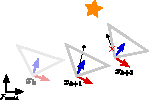
\includegraphics[width=0.65\columnwidth]{visibility.pdf} 
\caption{Forward propagation of the bearing vector to landmark $l$, originally detected at $\xhat_{k+1}$. Although $\xhatkkH$ contains the previous pose $\x_k$, the landmark was not detected there and so it is not considered. In this illustration, the predicted feature vector at $\xhat_{k+2}$ lies outside the field of view and so fails the visibility check.}
\label{fig:visibility}
\end{figure}

By stacking~\eqref{eqn:vision-model} row-wise for each time step in the horizon, we have the following compact model for how the $l$-th landmark detected at $k+1$ propagates throughout the horizon
\begin{equation}\label{eqn:vision-model-stacked}
\zl = \F_l\xhatkkH + \E_l\pWL + \nl,
\end{equation}
where $\zl\in\mathbb{R}^{3H}$, $\F_l\in\mathbb{R}^{3H\times 9(H+1)}$, and $\E_l\in\mathbb{R}^{3H\times 3}$.
However, in order for a point to be useful, it must be able to be triangulated (i.e., it must be seen from multiple time steps).
Any rows that correspond to poses for which the landmark was not seen are removed to prevent rank deficiency.
The final dimensions are then $\zl\in\mathbb{R}^{3n_\ell}$, $\F_l\in\mathbb{R}^{3n_\ell\times 9(H+1)}$, and $\E_l\in\mathbb{R}^{3n_\ell\times 3}$, where $n_\ell$ is the number of frames that landmark $l$ is visible.

We wish to identify the amount of information that the landmark $\pWL$ adds to the state estimation task.
Because $\pWL$ is not part of our state vector $\xhatkkH$, we first compute the information matrix of the joint state $\begin{bmatrix}\xhatkkH&\pWL\end{bmatrix}$ and then use the Schur complement to marginalize out the dependence on $\pWL$ and dispersing its information into the other states:
\begin{equation*}
\OmegakkH^{(l)} =
\begin{bmatrix}
\F_l^\top\F_l & \F_l^\top\E_l \\
\E_l^\top\F_l & \E_l^\top\E_l
\end{bmatrix}
\in\mathbb{R}^{9(H+1)+3\times9(H+1)+3}.
\end{equation*}
The Schur complement of $\OmegakkH^{(l)}$ is computed as
\begin{equation}\label{eqn:schur}
\Delta_l = \F_l^\top\F_l - \F_l^\top\E_l(\E_l^\top\E_l)^{-1}\E_l^\top\F_l \in\mathbb{R}^{9(H+1)\times9(H+1)},
\end{equation}
which gives the additive contribution of anticipated information from the $l$-th feature to our state estimate and is used in the greedy algorithm.

\subsubsection{Implementation Details}
Noting that the matrices in~\eqref{eqn:vision-model-stacked} are sparse, we can avoid large matrix multiplication by exploiting the sparsity patterns and reusing computation where possible.
The stacked matrices $\F_l$ and $\E_l$ have the following structure (before removing degenerate rows):
\begin{align}
\F_l &=
\begin{bmatrix}
\zero_{3\times9} & \A_{k+1,l} & \zero_{3\times9} & \cdots & \zero_{3\times9} \\
\zero_{3\times9} & \zero_{3\times9} & \A_{h,l} & \cdots & \zero_{3\times9} \\
\zero_{3\times9} & \zero_{3\times9} & \zero_{3\times9} & \ddots & \zero_{3\times9} \\
\zero_{3\times9} & \zero_{3\times9} & \zero_{3\times9} & \cdots & \A_{k+H,l} \\
\end{bmatrix}\\
\E_l &=
\begin{bmatrix}
-\B_{k+1,l}\\
-\B_{h,l}\\
\vdots\\
-\B_{k+H,l}\\
\end{bmatrix},
\end{align}
where
\begin{align}
\A_{h,l} &= \begin{bmatrix}\B_{h,l} & \boldsymbol 0_{3\times 6}\end{bmatrix}\in\mathbb{R}^{3\times9}\\
\B_{h,l} &= [\uhl]_\times(\RWIh\RIC)^\top\in\mathbb{R}^{3\times3}.
\end{align}
Computing the information matrix of the joint state $\begin{bmatrix}\xhatkkH&\pWL\end{bmatrix}$ gives the following sub-blocks, where we have taken advantage of the sparsity of $\A_{h,l}$.
For simplicity of notation, we drop the subscripts of $\A_{h,l}$ and $\B_{h,l}$ and simply use $1,\dots,H$ to denote $k+1,\dots,H$:
\begin{align*}
\F_l^\top\F_l &=
\begin{bmatrix}
\g\zero_{9\times9}&\g\zero_{9\times9}&\g\cdots&\g\zero_{9\times9}\\
\g\zero_{9\times9}&\cob\A_1^\top\A_1&\cdots&\zero_{9\times9}\\
\g\zero_{9\times9}&\zero_{9\times9}&\ddots&\zero_{9\times9}\\
\g\zero_{9\times9}&\zero_{9\times9}&\zero_{9\times9}&\cor\A_H^\top\A_H\\
\end{bmatrix}\\
&=
\begin{bmatrix}
\g\zero_{9\times9}&\g\zero_{9\times3}&\g\zero_{9\times6}&\g\cdots&\g\zero_{9\times3}&\g\zero_{9\times6}\\
\g\zero_{3\times9}& \cob\B_1^\top\B_1   &\cob\zero_{3\times6} &\cdots   &\zero_{3\times3}&\zero_{3\times6}\\
\g\zero_{6\times9}& \cob\zero_{6\times3}&\cob\zero_{6\times6} &\cdots&\zero_{6\times3}&\zero_{6\times6}\\
&&&\ddots&&\\
\g\zero_{3\times9}&\zero_{3\times3}&\zero_{3\times6}&\cdots&\cor\B_H^\top\B_H   &\cor\zero_{3\times6}\\
\g\zero_{6\times9}&\zero_{6\times3}&\zero_{6\times6}&\cdots&\cor\zero_{6\times3}&\cor\zero_{6\times6}
\end{bmatrix}\\
\F_l^\top\E_l &= \begin{bmatrix} \g\zero_{9\times3}\\ \cob-\A_1^\top\B_1\\ \vdots\\ \cor-\A_H^\top\B_H\\ \end{bmatrix}
=
\begin{bmatrix} \g\zero_{9\times3}\\ \cob-\B_1^\top\B_1\\ \cob\zero_{6\times3}\\ \vdots\\ \cor-\B_H^\top\B_H\\ \cor\zero_{6\times3} \end{bmatrix}
= (\E_l^\top\F_l)^\top\\
\E_l^\top\E_l &=
\begin{bmatrix}
\B_1^\top\B_1 + \cdots + \B_H^\top\B_H
\end{bmatrix}
\end{align*}

With an understanding of the pattern that these matrices exhibit, we can then efficiently calculate $\Delta_l$ as follows.
First, we note that the second addend in the Schur complement in~\eqref{eqn:schur} has the following form:
\begin{flalign*}
&
\F_l^\top\E_l(\E_l^\top\E_l)^{-1}\E_l^\top\F_l = &\\
&\quad
\begin{bmatrix}
\g\zero_{9\times9}&\g\zero_{9\times3}&\g\zero_{9\times6}&\g\cdots&\g\zero_{9\times3}&\g\zero_{9\times6}\\
\g\zero_{3\times9}& \C_1\W\C_1^\top   &\zero_{3\times6} &\cdots   & \C_1\W\C_H^\top&\zero_{3\times6}\\
\g\zero_{6\times9}& \zero_{6\times3}&\zero_{6\times6} &\cdots&\zero_{6\times3}&\zero_{6\times6}\\
&\vdots&&\ddots&\vdots&\\
\g\zero_{3\times9}& \C_H\W\C_1^\top   &\zero_{3\times6} &\cdots   & \C_H\W\C_H^\top&\zero_{3\times6}\\
\g\zero_{6\times9}& \zero_{6\times3}&\zero_{6\times6} &\cdots&\zero_{6\times3}&\zero_{6\times6}\\
\end{bmatrix},
\end{flalign*}
where $\C_i=\B_i^\top\B_i$ and $\W=(\E_l^\top\E_l)^{-1}$ (which is only invertible if a landmark was seen by more than one future pose).
Therefore, the final form of $\Delta_l$ is
\begin{flalign}\label{eqn:delta-ell}
&
\Delta_l = &\\
&\quad
\begin{bmatrix}
\g\zero_{9\times9}&\g\zero_{9\times3}&\g\zero_{9\times6}&\g\cdots&\g\zero_{9\times3}&\g\zero_{9\times6}\\
\g\zero_{3\times9}& \C_1-\D_{11}   &\zero_{3\times6} &\cdots   & -\D_{1H}&\zero_{3\times6}\\
\g\zero_{6\times9}& \zero_{6\times3}&\zero_{6\times6} &\cdots&\zero_{6\times3}&\zero_{6\times6}\\
&\vdots&&\ddots&\vdots&\\
\g\zero_{3\times9}& -\D_{H1}   &\zero_{3\times6} &\cdots   & \C_H-\D_{HH}&\zero_{3\times6}\\
\g\zero_{6\times9}& \zero_{6\times3}&\zero_{6\times6} &\cdots&\zero_{6\times3}&\zero_{6\times6}\\
\end{bmatrix},\nonumber
\end{flalign}
where $\D_{ij}=\C_i\W\C_j^\top$.
Finally, we note that when the camera at pose $\xhat_h$ did not see the $l$-th landmark, the corresponding rows and columns are zeroed out because that landmark offers no information for those state estimates.
